\documentclass[12pt,a4paper,titlepage]{article}
\usepackage{lab_style}
\usepackage{pdfpages}
\usepackage{eso-pic}
\usepackage{graphicx}
\usepackage{float}
\newcommand\tab[1][1cm]{\hspace*{#1}}

\graphicspath{ {./} }
  
\begin{document}

\begin{titlepage}
\selectlanguage{english}

%----------------------------------------------------------------------------------------
% TITLE PAGE INFORMATION
%----------------------------------------------------------------------------------------
  \begin{center} % Center everything on the page

  %----------------------------------------------------------------------------------------
  % HEADING SECTIONS
  %----------------------------------------------------------------------------------------
  \textsc{\large Faculty of Computers, Informatics and Microelectronics}\\[0.5cm]
  \textsc{\large Technical University of Moldova}\\[1.2cm] % Name of your university/college
  \vspace{25 mm}

  \textsc{\Large Object-Oriented Modeling and Analysis}\\[0.5cm] % Major heading such as course name
  \textsc{\large Laboratory work \#9}\\[0.5cm] % Minor heading such as course title

\newcommand{\HRule}{\rule{\linewidth}{0.5mm}} % Defines a new command for the horizontal lines, change thickness here

  %----------------------------------------------------------------------------------------
  % TITLE SECTION
  %----------------------------------------------------------------------------------------
  \vspace{10 mm}
  \HRule \\[0.4cm]
  { \LARGE \bfseries Modeling your project with Deployment Diagrams. Data Flow Diagrams. OntoUML. }\\[0.4cm] % Title of your document
  \HRule \\[1.5cm]

  %----------------------------------------------------------------------------------------
  % AUTHOR SECTION
  %----------------------------------------------------------------------------------------
      \vspace{30mm}

      \begin{minipage}{0.4\textwidth}
      \begin{flushleft} \large
      \emph{Author:}\\
      Cernei \textsc{Liviu}
      \end{flushleft}
      \end{minipage}
      ~
      \begin{minipage}{0.4\textwidth}
      \begin{flushright} \large
      \emph{Supervisor:} \\
      Mihail \textsc{Gavrilița} % Supervisor's Name
      \end{flushright}
      \end{minipage}\\[4cm]

      \vspace{5 mm}
      % If you don't want a supervisor, uncomment the two lines below and remove the section above
      %\Large \emph{Author:}\\
      %John \textsc{Smith}\\[3cm] % Your name

      %----------------------------------------------------------------------------------------
      % DATE SECTION
      %----------------------------------------------------------------------------------------

      {\large Chișinau 2018}\\[3cm] % Date, change the \today to a set date if you want to be precise

      %----------------------------------------------------------------------------------------
      % LOGO SECTION
      %----------------------------------------------------------------------------------------

      %\includegraphics{red}\\[0.5cm] % Include a department/university logo - this will require the graphicx package

      %----------------------------------------------------------------------------------------

      \vfill % Fill the rest of the page with whitespace
      \end{center}
      
\end{titlepage}

\cleardoublepage

\newpage

\pagenumbering{arabic}
\setcounter{page}{1}
\setcounter{secnumdepth}{4}

\addtocontents{toc}{\protect\thispagestyle{empty}} % no page number on the table of contents page
\cleardoublepage


\phantomsection
\addcontentsline{toc}{section}{Introduction}
\section*{Laboratory work \#9}
\phantomsection

\section{Tasks}
\begin{itemize}
	\item
	Model your application using Deployment Diagrams;
	\item 
	Create an overview of your project using Data Flow Diagrams; Choose any standard
you like.
\end{itemize}

\section{Theory}

\subsection{OntoUML}
OntoUML is a pattern-based and ontologically well-founded version of the Unified Modeling Language (UML). Its meta-model has been designed in compliance with the ontological distinctions of a well-grounded theory, named the Unified Foundational Ontology (UFO). OntoUML includes a system of interrelated axiomatic theories, providing modeling foundations for all Conceptual Modeling major concepts, including theories for: types and taxonomic structures (including roles), part-whole relations, events, formal and material relations, dependent (weak) entities, attributes and attribute value and measurement spaces (roughly datatypes). \par

OntoUML (and its foundations) has been adopted by many institutions worldwide (in academia, industry and government). In particular, OntoUML has been considered as a candidate for addressing the OMG SIMF (Semantic Information Model Federation) Request for Proposals after a report of its successful use over the years by a department of the U.S. Department of Defense (DoD)\par
\clearpage

\section{Deployment Diagrams}
In Figure ~\ref{fig:deploy} is represented the deployment diagram for the app.
\begin{figure}[H]
\centering
	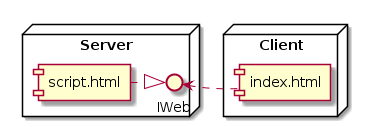
\includegraphics[width=10cm]{deploy}
	\caption{Website deployment diagram}
	\label{fig:deploy}
\end{figure}

\section{Data Flow Diagram}
In Figure ~\ref{fig:data} is represented the Data-Flow diagram for the app.
\begin{figure}[H]
\centering
	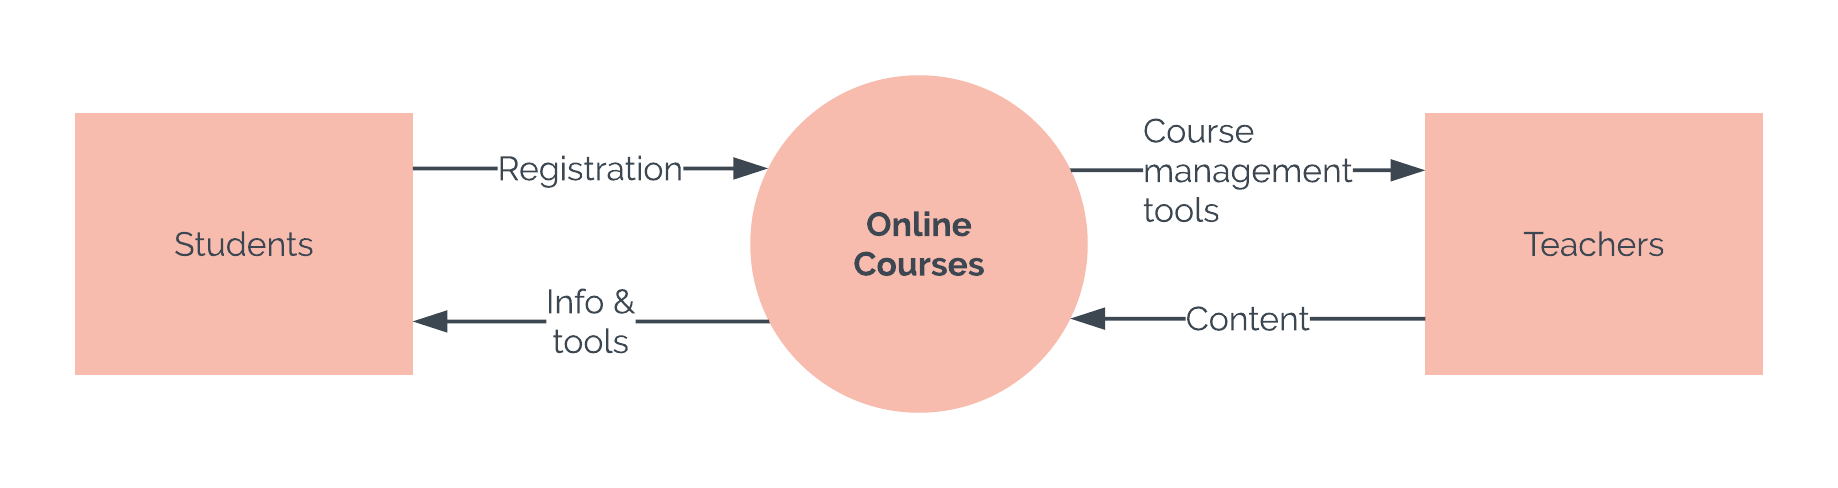
\includegraphics[width=15cm]{data}
	\caption{Website Data Flow Diagram}
	\label{fig:data}
\end{figure}

\section{Conclusion}
In this laboratory work we learned to create Deployment and Data Flow diagrams.

\clearpage
\cleardoublepage

\end{document}
